\documentclass{beamer}
% \documentclass[handout,xcolor=pdftex,dvipsnames,table]{beamer}
% \documentclass[draft]{beamer}
% \includeonlyframes{current,curr2}
\usepackage{enumerate}
\usepackage{hyperref}
\usepackage{amsmath}
\usepackage{amsthm}
\usepackage{amssymb}
\usepackage{amsfonts}
\usepackage{pdfpages}
\usepackage{booktabs}
\usepackage{nccmath}
\usepackage{bbm}

\usetheme{Boadilla}

\hypersetup{%
	pdftitle={Slides},%
	pdfauthor={James G. Partridge},%
	pdfsubject={},%
	pdfkeywords={Firm Capital, Credit Rating Agencies, Macro, School}%
}

\newtheorem{prop}[theorem]{Proposition}

\title[Information, Ratings and Corporate Bonds]{The Role of Public Information and Credit Ratings\\in the Corporate Bond Market}
\author[JGP]{James Partridge} 
\institute[UWO]{The University of Western Ontario}
\date[August 18, 2012]{Macro Lunch} 

\begin{document}

\begin{frame}{Puzzling Observation}
\begin{itemize}
	\item Number of AAA firms (S\&P): now 4, down from 34 in 1985!
	\item Number of AAA and AA rated firms have decreased, while the total number of firms with a rating has increased. 
\end{itemize}
\vspace{0.35cm}
\hspace{0.8cm}\textbf{Question:} \\
\hspace{0.8cm}Why have so many high rated firms disappeared? \\
\vspace{0.5cm}

\begin{quote}
Scores of big companies have lost their AAA status in recent years as it became seen in board rooms as more of a straitjacket than a path to riches.\\
\hspace*\fill \textup{\footnotesize{Eric Dash, New York Times, August 2, 2011}}
\end{quote}

\hspace{0.8cm}\textbf{My conjecture:} \\
\begin{quote}
Ratings have value as a signal, but this value has diminished as information proliferation has increased.
\end{quote}

\end{frame}

\begin{frame}{Story}
\begin{itemize}
	\item \alert<1>{Then:} CRA ratings were the primary source of firm information, few had access to SEC filings, firm prospectus,\ldots
	\item \alert<1>{Now:} Bloomberg, WSJ Online, etc. all provide market data and firm analysis; firm info is readily available
	\item Rating and third-party market analysis both act as signals of firm's well-being or quality
	\item Cost required to achieve high ratings
\end{itemize}
\begin{quote}
Investors now have direct information on firm quality -- \\ high quality firms no longer willing to incur cost of high ratings
\end{quote}
\end{frame}

\begin{frame}{Environment}
\begin{itemize}
	\item Firms are of \textbf{type} $\theta \epsilon \left\{g,b\right\}$, unobserved by all
	\begin{itemize}
		\item determines probability the firm's project is successful
	\end{itemize}
	\item Economy receives a \textbf{signal}, $\nu \epsilon \left\{h,l\right\}$, about firm's type
	\begin{itemize}
		\item probability signal is `accurate' is $\omega$
		\item assume $\omega > 0.5$
	\end{itemize}
	\item The firm chooses resources to devote to the rating process, economy then observes \textbf{rating}, $\kappa \epsilon \left\{A,B,C\right\}$
	\begin{itemize}
		\item accuracy of rating depends on investment
	\end{itemize}
\end{itemize}
\end{frame}

\begin{frame}{Timing}
\begin{enumerate}
	\item Ex ante:
	\begin{itemize}
		\item known: public signal ($\kappa$ or $l$)
		\item unknown: type ($g$ or $b$)
	\end{itemize}
	\item Interim:
	\begin{itemize}
		\item firm chooses $i$
		\item rating is formed and observed ($A$, $B$ or $C$)
		\item debt contracts are issued, interest rates conditioned on $\kappa$ and $\nu$
	\end{itemize}
	\item Ex post:
	\begin{itemize}
		\item outcome of project is realized (0 or $y$)
		\item debt is paid if project pays off
	\end{itemize}
\end{enumerate}
\end{frame}

\begin{frame}{Model}
\begin{itemize}
	\item Firms:
	\begin{itemize}
		\item endowed with a project that might earn $y$ if investment is received
		\item project requires investment $d=1$, fixed
		\item $\mathbbm{1}(\kappa,\nu)=1$ if investment is received, 0 otherwise
	\end{itemize}
\end{itemize}
\begin{equation}
	\label{eq:FP}V(\nu)=\max_{i} \,\,\, -c(i)+\textup{E}_{\theta,\kappa}\left [ \mathbbm{1}(\kappa,\nu) \left (y - R(\kappa,\nu) \right )|\nu\right ]
\end{equation}
\begin{itemize}
	\item Investors:
	\begin{itemize}
		\item investors observe $\nu$ and $\kappa$
		\item have access to risk free outside option which pays $r$
		\item expected return is then:
	\end{itemize}
\end{itemize}
\begin{equation}
	\textup{E}_{\theta} \left [R(\kappa,\nu)|\kappa,\nu \right ]
\end{equation}
\end{frame}


\begin{frame}{Price Dispersion}
\begin{itemize}
	\item As information proliferates bond prices are affected
	\begin{itemize}
		\item Investors condition on ratings \textit{and} public information
	\end{itemize}
	\item Standard deviation of bond prices increasing for each rating class...
	\begin{itemize}
		\item but so is the mean...
		\item so use coeffecient of variation (CV) instead
	\end{itemize}
	\item Can test for statistical significance
	% \begin{itemize}
		% \item Need assumption of log-normality
	% \end{itemize}
\end{itemize}
\end{frame}

{
\setbeamercolor{background canvas}{bg=}
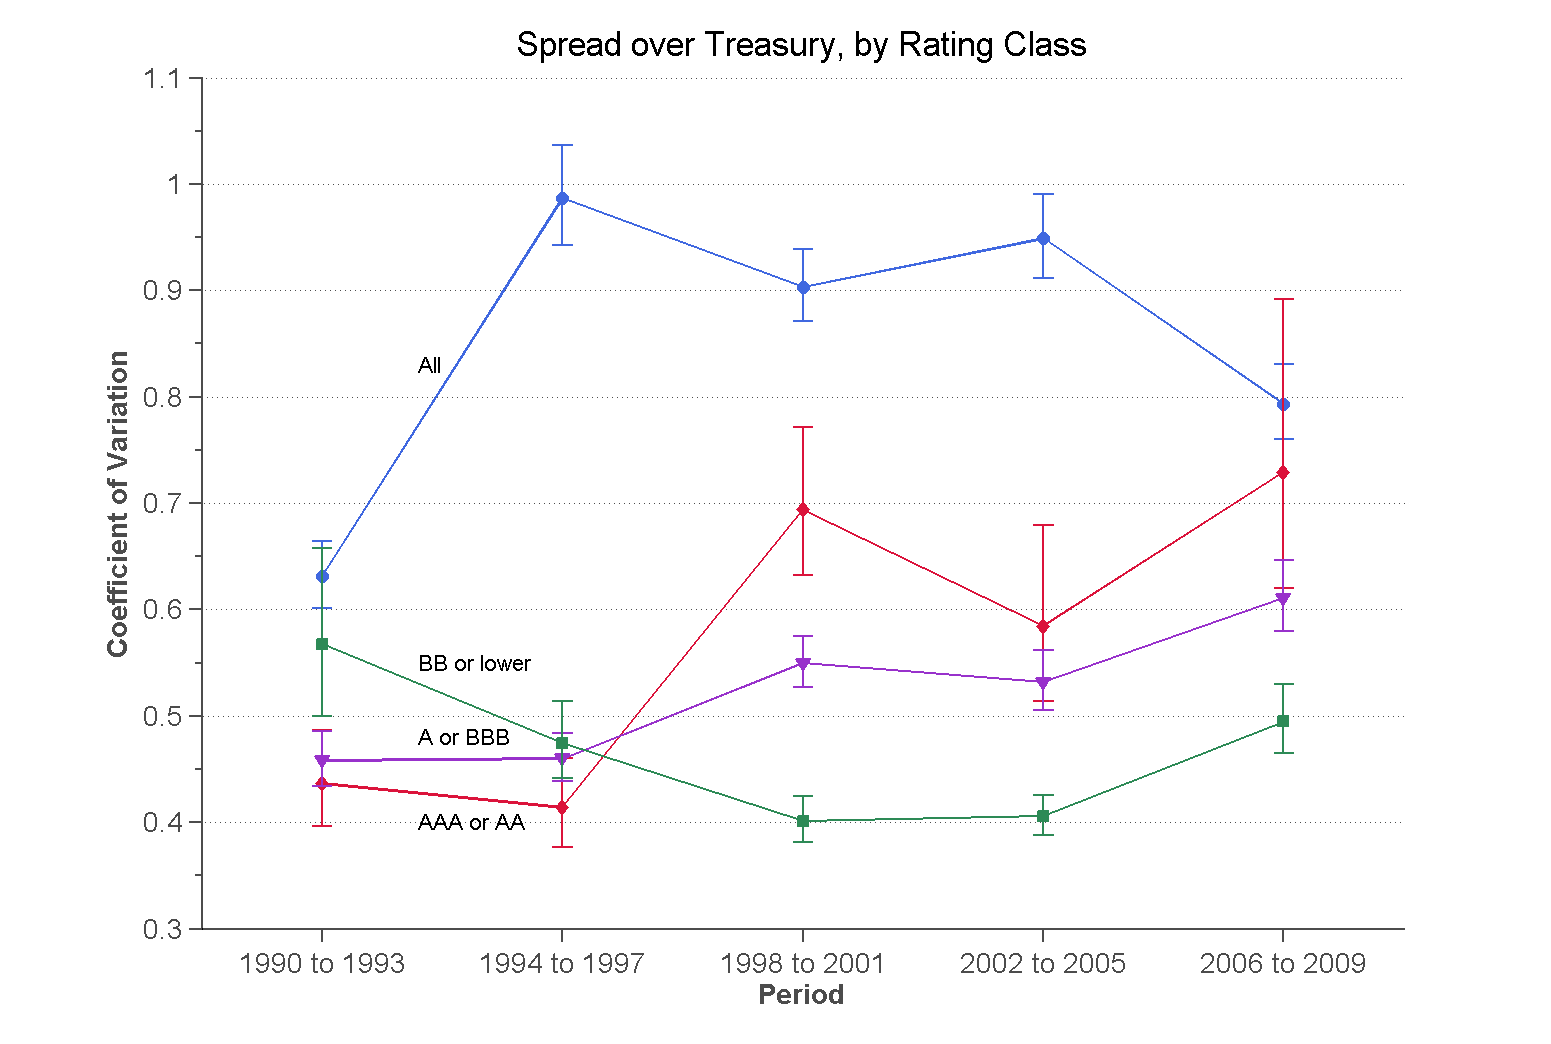
\includepdf{CVCI.png}
}

\end{document}

